\documentclass[10pt,technote]{IEEEtran}
\usepackage[utf8]{inputenc}
\usepackage{amsmath}
\usepackage{amsfonts}
\usepackage{amssymb}
\usepackage{multicol}
\usepackage{csquotes}
\usepackage{graphicx}
\usepackage[T1]{fontenc}
\usepackage{algorithm}
\usepackage{algpseudocode}
\author{B. I. Lyons \quad J. Michael Herrmann}
\title{The Role of Reflexive Reinforcement Learning in Solutions to the Inverse Problem}
\begin{document}
\maketitle
\begin{abstract}
Inverse reinforcement learning is an ill-defined problem because multiple reward functions can represent the displayed policy, as such a demonstrating agent must be able to reactively alter its behaviour to demonstrate effectively to an observer. We show here that employing the learner's belief as a reflexive component allows for a clearer image of the reward function from the demonstrator under the the maximum entropy inverse reinforcement learning paradigm, allowing for the possibility of robot and computational agents demonstrating tasks to human agents, as well as having potential ramifications for explainable AI.
\end{abstract}

\section{Introduction}

Reinforcement learning (RL)~\cite{sutton2018reinforcement} has consistently proven itself in a wide variety of simulated tasks, and important intelligence milestones, from competing at a level superior to the greatest human players in traditional board games~\cite{campbell2002deep, silver2017mastering}, and competing at an expert level or greater in computer games of varying complexity~\cite{berner2019dota, mnih2013playing}, as well as the learning of complex behaviours in real robot platforms~\cite{andrychowicz2020learning, morimoto2001acquisition, asada1996purposive, karnchanachari2020practical} and yet, real world applications of reinforcement learning are few and far between.

Challenges that impact the implementations of real-world RL are varied, though some of the most commonly cited issues are:

\begin{itemize}
\item Learning time is impractical, the agent must be able to learn on the real system from a limited number of samples;
\item Safety is of paramount importance, and trial and error learning can result in dangers to both the machine and humans in contact with the agent;
\item Desires for explainable policies and actions;
\item Reward functions that result in representations of the value function which are close to the true value function are hard to define and can result in unforseen abuses of the environment and behaviours which are undesirable.
\end{itemize}

In recent years, in an attempt to solve or mitigate some or all of these issues, greater interest has been placed in the subfield of RL, \emph{imitation learning}, in which an agent attempts to learn the task either being operated by an expert, or by observing an expert and attempting to replicate the behaviour. One of the most promising avenues for this has been research into inverse reinforcement learning (IRL)~\cite{ng2000algorithms}, in which, an agent attempts, from a collection of trajectories assumed to be near optimal, to reconstruct the reward function implied by the action selection in the state. The motivations for inverse RL are clear both within the field of computer science, and without:

\begin{itemize}
\item Modeling of animal and human behaviour for the purposes of scientific enquiry, e.g. if inverse RL is possible we may be able to determine the reward functions utilised by animal behaviours such as foraging and vocalisation in bees and songbirds respectively~\cite{ng2000algorithms};
\item Imitation learning through inverse reinforcement learning such that an agent can learn over a smaller number of samples and at a reduced risk to both itself and humans in the loop;
\item Modelling other agents in the environment in which the agent exists, both adversarial and cooperative, which may lead to a better foundation for multi agent tasks.
\end{itemize}

Whilst IRL is highly promising, it is not without serious drawbacks of its own. It has been noted by many within the field of RL to be an \emph{ill-posed problem}~\cite{abbeel2004apprenticeship, ziebart2008maximum, choi2011inverse}, both due to its nature, as well as being computationally intractable, where many possible reward functions can represent the supplied trajectories, and the difficulty of solving partially observable Markov decision processes (POMDP) with a belief state.

It is our research aim to address some of these issues inherent in the IRL problem with our own approach to reinforcement learning, \emph{reflexive reinforcement learning} (RRL)~\cite{ncta20}, in which an agent is able to adapt its behaviour episode by episode, using a reflexive reward in addition to the task reward, such that it performs the task at a sub-optimal level whilst demonstrating the task to another agent. These tasks have been performed in gridworld environments with the aim to be extended in future work. This instantiation of the RRL paradigm is denoted IRL-RRL, due to using IRL generated information as a reflexive component.

The rest of this paper is organised as follows, in Sect.~\ref{sect:background} we will discuss the inverse reinforcement learning problem, specifically maximum entropy inverse reinforcement learning, the DynaQ and DynaQ+ architechtures, as well as the RRL paradigm. In Sect.~\ref{sect:methods} we discuss the experimental setup, and the metric we use for analysis, before discussing results in Sect.~\ref{sect:results}. Applications, conclusions, and future work will be discussed in Sections~\ref{sect:applications}, \ref{sect:conclusions}, \ref{sect:future} respectively.

\section{Background} \label{sect:background}

\subsection{Preliminaries} \label{subsect:prelim}

A finite Markov decision problem (MDP) is a tuple, $(X, A, T, D, R)$, where $X$ is a finite set of states, $A$ a finite set of actions, $T= {P_{x,a}}$ such that $P_{x,a}$ is the distribution when taking action $a$ in state $x$, $D$ is the initial-state distribution from which the initial state $x_0$ is drawn, and $R$ is a function that assigns to each state-action pair\footnote{or possibly to triplets: state, action and following state} a number $r$ (or a random variable with mean $r$) which provides a direct or delayed (stochastic) evaluation of this pair.

The RL agent then aims at finding solutions to the Bellman problem of reconstructing a value function that obeys
\begin{equation}
	V^*(x)=\max_a \left(R(x,a) + \gamma \sum_{x'} P(x'|x,a) V^*(x')\right)
\end{equation} 
where $x$ is the current and $x'$ the subsequent state, and action $a$ is executable in state $x$.

This task can be achieved by the assumption that there exists some function $Q^* (x,a)$ which is the value of taking an action in a given state, and that contains the information about the expected reward. In this function approximation approach, we aim to adjust our policy $\pi$ such that $Q^* (x,a) \leftarrow Q^\pi (x,a), V^* (x) \leftarrow Q^\pi (x)$ by defining them as
\begin{eqnarray}
	Q^\pi (x,a)&=&E\left[\sum_{t=0}^\infty\gamma^{t} r_t| x_0 = x, a_0 = a \right]\\
	V^\pi (x)&=&E\left[\sum_{t=0}^\infty\gamma^{t} r_t | x_0 = x \right] 
\end{eqnarray}
where $Q^\pi (x,a)$ is updated by~\cite{sutton1999reinforcement}
\begin{equation} \label{faeqn}
Q^\pi(x,a) = \alpha \left(r_t + \gamma V(x_{t+1}) -  Q(x,a) \right)
\end{equation}
with discount $\gamma$ and learning rate $\alpha$ and the value is given by
\begin{equation}
	V^\pi (x_{t+1})=\max_a Q^\pi (x_{t+1},a).
\end{equation}
the resulting effect is that the trial and error nature results in $t\rightarrow \infty, Q^\pi(x,a) \rightarrow Q^*(x,a), V^\pi(x) \rightarrow V^*(x)$.

\subsection{Inverse Reinforcement Learning}

In the case of the IRL problem, we consider an MDP without a reward function, by convention denoted MDP\textbackslash R, i.e., a tuple of the form $(X, A, T, D)$. We then make some basic assumption: $(1)$ that there exists some function $\phi (x_i) : x_i \rightarrow \textbf{f}_{x_i}$ which linearly maps $x_i \in X$ to some features of the state $\textbf{f}_{x_i} \in [0, 1]^k$, where $k$ is the number of features; $(2)$ there exists some reward function $R^*(x) = w^* \cdot \phi(x)$, where $w^* \in \mathbb{R}^k$ are the reward weights.

The setup then is that there is an (assumed) expert agent which generates trajectories, $\zeta$ in each episode, consisting of states $x_i$ and actions $a_i$, where $i= 1,..., t$, where $t$ is the length of the episode, and is not necessarily of constant length. Thus, the reward value of a trajectory is the sum of the state rewards

\begin{equation} \label{eqn:traj_reward}
R*(\textbf{f}_\zeta) = \sum_{x_i \in \zeta} {w^{*}}^\top \textbf{f}_{x_i}
\end{equation}
with empirical feature count
\begin{equation}
\mathbb{E}[\textbf{f}] = \frac{1}{N} \sum_{i}^{N} \textbf{f}_{\zeta_i}
\end{equation}

Observing the above it becomes readily apparent that this is an ill-posed problem, as many reward weights will result in the demonstrated trajectories being optimal.

As an alternative, it was proposed in \cite{abbeel2004apprenticeship} to instead match \emph{feature expectations} estimated by
\begin{equation}
\hat{\mu} (\pi) = \frac{1}{N} \sum_{i}^{N} \sum_{t} \gamma^t \textbf{f}_t
\end{equation}
between an observed policy $\pi$ and an agents behaviour, where $\gamma$ is the discount factor, and $t$ is the time step in a given trajectory. Despite this improvement, the problem remains, in that each policy can be optimal for many reward functions, and many policies will lead to the same feature counts.

\subsection{DynaQ and DynaQ+}

DynaQ \cite{sutton1991integrated} was first proposed as an extension of the RL architecture such that an agent is able to generate hypothetical experience from the model that it builds throughout the learning phase, these can be thought of as planning steps, as in a the traditional approach, an $\varepsilon$-greedy agent builds one step of a policy during each episode. 

These hypothetical simulated experiences, recorded in the model, acting as a form of memory, allows the agent to reinforce its belief in good state-action values in an earlier phase of the learning process, converging to greater task performance much earlier.

\begin{algorithm}
\caption{DynaQ}
\begin{algorithmic}[1]
\Require Initialise $Q(x,a),Model(x,a) \forall x \in X, a \in A$, and planning steps $N \in \mathbb{N}$ 
\While{$t<\infty$}
\State $x_t \leftarrow$ current (nonterminal) state
\State $a_t \leftarrow$ $\varepsilon$-greedy$(x_t,Q)$
\State Take action $a_t$; observe new state $x_{t+1}$ and reward $r_t$
\State $Q(x,a) \leftarrow \alpha \left(r_t + \gamma V(x_{t+1}) -  Q(x,a) \right)$
\State $Model(x_t,a_t) \leftarrow r_t, x_{t+1}$ (assuming deterministic)
\State $n=0$
\While{$n<N$}
\State $x_n \leftarrow$ random previously observed state
\State $a_n \leftarrow$ random previously observed action
\State $r_t, x_{t+1} \leftarrow Model(x_t,a_t)$
\State $Q(x,a) \leftarrow \alpha \left(r_t + \gamma V(x_{t+1}) -  Q(x,a) \right)$
\State $n \leftarrow n+1$
\EndWhile
\EndWhile
\end{algorithmic}
\label{alg:dynaq}
\end{algorithm}

In the same paper, Sutton goes on to discuss DynaQ+ in which the agent extends the model to count when a previous state-action pair was previously attempted, providing a small exploration bonus to the reward in $Q$-update of the planning steps in Algorithm~\ref{alg:dynaq}, such that if a state has not been visited in some time, it will become more appealing if sampled in this loop, encouraging continued exploration in potentially changing environments.

\begin{algorithm}
\caption{DynaQ+}
\begin{algorithmic}[1]
\Require Initialise $Q(x,a),Model(x,a) \forall x \in X, a \in A$, and planning steps $N \in \mathbb{N}, \tau(x,a)$ as a function of time since action $a$ taken in state $x$ and $\kappa$ small. 
\While{$t<\infty$}
\State $x_t \leftarrow$ current (nonterminal) state
\State $a_t \leftarrow$ $\varepsilon$-greedy$(x_t,Q)$
\State Take action $a_t$; observe new state $x_{t+1}$ and reward $r_t$
\State $Q(x,a) \leftarrow \alpha \left(r_t + \gamma V(x_{t+1}) -  Q(x,a) \right)$
\State $Model(x_t,a_t) \leftarrow r_t, x_{t+1}$ (assuming deterministic)
\State $n=0$
\While{$n<N$}
\State $x_n \leftarrow$ random previously observed state
\State $a_n \leftarrow$ random previously observed action
\State $r_t, x_{t+1} \leftarrow Model(x_t,a_t)$
\State $r_t \leftarrow r_t + \kappa \sqrt{\tau}$ 
\State $Q(x,a) \leftarrow \alpha \left(r_t + \gamma V(x_{t+1}) -  Q(x,a) \right)$
\State $n \leftarrow n+1$
\EndWhile
\EndWhile
\end{algorithmic}
\label{alg:dynaq}
\end{algorithm}

\subsection{Maximum Entropy Inverse Reinforcement Learning}

In an effort to resolve the ambiguities inherent in the IRL problem, Ziebart et al.~\cite{ziebart2008maximum} utilise maximum entropy to reduce to a single stochastic policy over feature counts.

\begin{eqnarray}
P(\zeta | w^*, T)&=&\sum_{o \in \mathcal{T}} P_T (o) \frac{e^{w*^{\top} \textbf{f}_\zeta }}{Z (w^*, o)} I_{\zeta \in o} \\
&\approx & \frac{e^{w*^{\top} \textbf{f}_\zeta }}{Z (w^*, T)} \prod_{x_{t+1}, a_{t+1}, x_t \in \zeta} P_T (x_{t+1} | a_{t}, x_{t})
\end{eqnarray}
with
\begin{equation}
P(a | w^*, T) \propto \sum_{\zeta : a \in \zeta_{t=0} }P (\zeta | w^*, T)
\end{equation}

\subsection{Reflexive Reinforcement Learning}

RRL considers that the vast quantity of information generated over the learning process has significant value, and that reduction to some pure task policy is a hindrance in attempts at autonomous, continuous learning of an agent. Instead, by utilising a \emph{reflexive component} which adapts the reward signal between the environment and the agent, the state valuation can be informed by other information, with the intention of generating behaviours and valuations which represent the states beyond just a task. Previously we have shown that we are able to generate empowerment~\cite{klyubin} like quantities on-line~\cite{ncta20}.

Although in this instance we utilise the $Q$-learning algorithm as outlined in Sect.~\ref{subsect:prelim}, as RRL adjusts the reward signal based on some predetermined criteria, it has the advantage of being compatible with other approaches to RL, as well as being highly flexible.

We believe RRL to be a good approach to improving the efficacy of IRL, as an agent that is ``educating" another agent by supplying trajectories should not simply provide the optimal policy, but must instead attempt to accurately depict the reward function of the environment. As such this means continuously adapting its behaviour over a set of trajectories such that the output of the Max Ent IRL algorithm best represents the true reward function, whilst also continuing to perform the task to completion.

\section{Methods} \label{sect:methods}

To demonstrate the ability for a learning agent to be an accurate demonstrator of a multi-reward environment, our greedy agent performs a given task with two rewards, in this instance the task is to attend one of the terminal absorbing states.

Following the completion of each episode, a separate agent performs Maximum Entopy IRL over the trajectories supplied so far to generate a belief of the reward function of the environment.

\subsection{Environment}

\subsubsection{2D World}

The 2D world environment is a discrete world $N$x$N$ world, with two to four terminal, reward states at each corner of the state space. In each instance the rewards are determined to be $r_1 \leq r_2$.

\subsubsection{Actions and Policy}

The agent has four possible actions, consisting of moves in each of the cardinal directions, it cannot remain in the same state with the exception of moving into the walls at the edge of the environment.

The agent draws its actions using softmax action selection using a Boltzmann distribution:
\begin{equation}
p(a|x) = \frac{e^{Q_t (a|x) / \tau}}{\sum^{A}_{b=1}e^{Q_t (b|x) / \tau}}
\end{equation}
where $\tau$ is the temperature, and $Q_t (a|x)$ and $Q_t (b|x)$ are the $Q$-values for actions $a$ and $b$ in state $x$ respectively. For our experiments we opted to use $\tau=10$.


\subsection{Reflexive Component}

Much like in the case of DynaQ+ we consider the case of implementing temporal information into the model to encourage non-optimal behaviour in future tasks to adjust for the inverse learners belief.

\begin{algorithm}
\caption{IRL-RRL}
\begin{algorithmic}[1]
\Require Initialise $Q(x,a) \forall x \in X, a \in A$, and planning steps $N \in \mathbb{N}$ 
\While{$e<E$}
\While{$x_t$ not terminal}
\State $x_t \leftarrow$ current (nonterminal) state
\State $a_t \leftarrow$ $p(a|x, \tau)$
\State Take action $a_t$; observe $x_{t+1}$ and reward $r_t$
\State $Q(x,a) \leftarrow \alpha \left(r_t + \gamma V(x_{t+1}) -  Q(x,a) \right)$
\State Store trajectory $[(x_i, a_i), ..., (x_T, a_T)]$
\EndWhile
\State Receive IRL belief from observer, $I(x) \forall X$
\State $n=0$
\While{$n<N$}
\State $x_n \leftarrow$ random previously observed state
\State $a_n \leftarrow$ random previously observed action
\State $r_t, x_{t+1} \leftarrow R(x) - I(x)$
\State $Q(x,a) \leftarrow \alpha \left(r_t + \gamma V(x_{t+1}) -  Q(x,a) \right)$
\State $n \leftarrow n+1$
\EndWhile
\EndWhile
\end{algorithmic}
\label{alg:irlrrl}
\end{algorithm}

The intent here is that, using the difference between what the educating robot knows to be true and the observer's belief, the teaching agent will be more likely to attend or avoid states which are falsely believed to be too low or too valuable respectively.

\subsection{Success Metrics}

Mean sqyared error below 0.01

\section{Results} \label{sect:results}

\begin{figure}[!t]
\centering
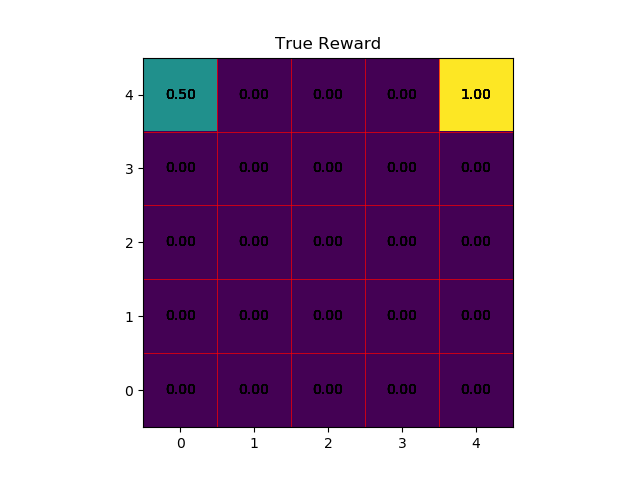
\includegraphics[width=2.5in]{pics/True_Reward.png} 
\end{figure}

\begin{figure}[!t]
\centering
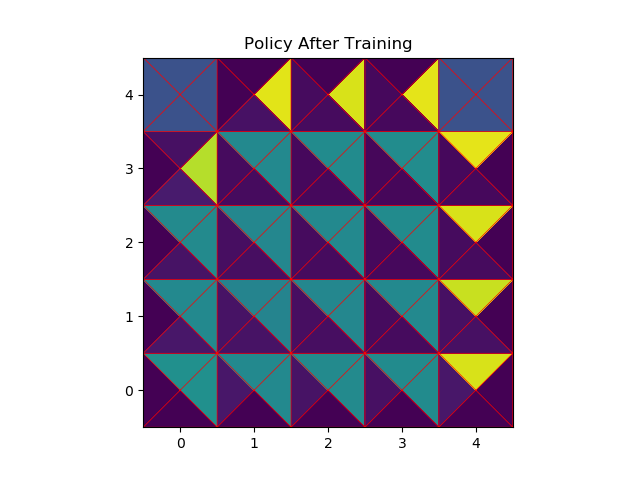
\includegraphics[width=2.5in]{pics/After_training.png} 
\end{figure}

\section{Applications} \label{sect:applications}

\subsection{Rapid Prototyping}
Robots teaching robots, minor changes as such state space likely transferrable between. Different embodiments etc. etc.

\subsection{Explainable AI}
Given an agent learns some task via a black box method such as ANNs it should be able to display substandard behaviours and by comparison we should observe what it has learned about the space in a less abstract way - Unsure. Robots teaching people

\subsection{Multi agent systems}
Adversarial, cooperative and neutral agents able to identify one another more succinctly by altering performance to display "what they are".???


\section{Conclusions} \label{sect:conclusions}

\section{Future Work} \label{sect:future}

\bibliographystyle{plain}
\bibliography{irlassistance.bib}
\end{document}